\section{Executive summary}

The \pmu at \kispi is proposed to represent the forefront of medical science, using an integrated multi-omics approach to augment paediatric healthcare. 
This strategy extends beyond genomic data to incorporate a wide array of omics technologies, such as genomics, proteomics, metabolomics, and innovative methods like single-cell sequencing. 
Together, these technologies  can provide a comprehensive understanding of disease mechanisms, which is instrumental in devising personalised treatment strategies for rare and complex paediatric conditions.

Comparable benchmarks have demonstrated clear cost-saving potential through precise diagnostics and targeted therapy.
For rare diseases, approximately 40\% of probands received a genetic diagnosis 
\citep{wright2023genomic, wojcik2024genome}
and altered critical care management in 77\% of diagnosed cases \citep{lunke2023integrated}.
A well-managed work-flow can result in rapid whole-genome sequencing with a turnaround of 37 hours on average
 \citep{abou2023rapid}.
A forecast, projected into 2030, for the yearly cases of sepsis are shown in 
\textbf{figure
\ref{fig:p_cases_sepsis_kispi_yearly_forecast_exec}}.
Black and red values show the expected number of deaths with and without  precise diagnostics and targeted therapy, respectively. 


Establishing these benchmarks as our initial goals is not only technically feasible but also a significant achievement in its own right, setting a foundation for potential further advancements as our understanding and capabilities evolve.

\begin{figure}[h] \hspace*{0cm} 
\begin{center}
	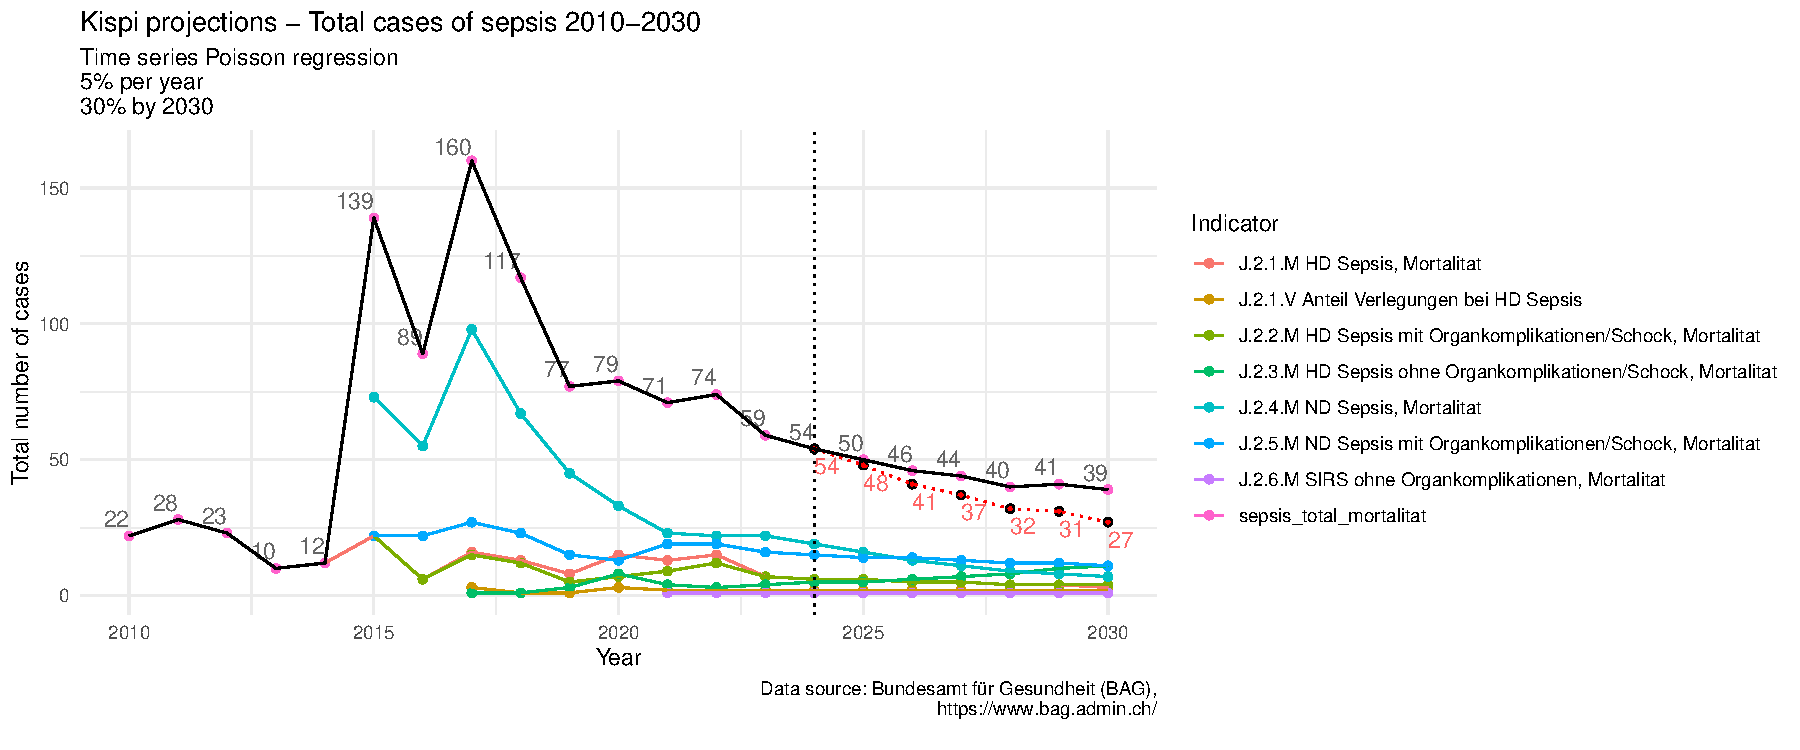
\includegraphics[width=1\textwidth]{../stats/foph_key_stats/output/p_cases_sepsis_kispi_yearly_forecast}
	\caption{Year deaths due to sepsis at \kispi.
	This data is based on statistics reported by Bundesamt für Gesundheit (BAG), 
	\url{https://www.bag.admin.ch/} for years 2010-2022. 
	Time series was performed using Poisson regression to extrapulate the expected outcomes from 2010-2030.
	Predictions for the cost and number of cases were generated in section 
	\ref{sec:benefit_analysis}.	
	DP: Diagnostic procedure.
HD: Primary diagnosis.
ND: Secondary diagnosis.
}
	\label{fig:p_cases_sepsis_kispi_yearly_forecast_exec}
\end{center}
\end{figure}























